\section{Configuring the system}

\begin{frame}
	\frametitle{Configuration}
	\begin{itemize}
		\item The Linux Kernel has a lot of available configurations
		\item Some are dedicated to performance
			\begin{itemize}
				\item Focus on improving the most-likely scenario
				\item Have the best average performance
				\item Optimize throughput and low-latency
				\item Usually have a slow-path, which is non-deterministic
			\end{itemize}
		\item Some are dedicated to security and hardening
		\item Some can be useful for Deterministic Behaviour
	\end{itemize}
\end{frame}

\begin{frame}
	\frametitle{CPU Pinning}
	\begin{itemize}
		\item The Linux Kernel Scheduler allows setting constraints about the CPU cores that are allowed
			to run each task
		\item This can be useful for lots of purposes:
			\begin{itemize}
				\item Make sure that a process won't be migrated to another core
				\item Dedicate cores for specific tasks
				\item Optimize the data-path if a process deals with data handled by a specific CPU core
				\item Ease the job of the scheduler's CPU load-balancer, whose complexity grows non-linearly with the number of CPUs
			\end{itemize}
		\item This mechanism is called the \code{cpu affinity} of a process
		\item The \code{cpuset} subsystem and the \code{sched_setaffinity} syscall are used to select the CPUs
		\item Use \code{taskset -p <mask> <cmd>} to start a new process on the given CPUs
	\end{itemize}
\end{frame}

% isolcpus
\begin{frame}
	\frametitle{CPU Isolation}
	\begin{itemize}
		\item Users can pin processes to CPU cores through the cpu affinity mechanism
		\item But the kernel might also schedule other processes on these CPUs
		\item \code{isolcpus} can be passed on the kernel commandline
		\item Isolated CPUs will not be used by the scheduler
		\item The only way to run processes on these CPUs is with cpu affinity
		\item Very useful when RT processes coexist with non-RT processes
	\end{itemize}
	\code{isolcpus=0,2,3}
\end{frame}

\begin{frame}
	\frametitle{CPU Isolation - cpusets}
	\begin{itemize}
		\item \code{cpuset} is a mechanism allowing to subdivide the CPU scheduling pool
		\item They are created at runtime, through the \code{cpusetfs}
			\begin{itemize}
				\item \code{mount -t cpuset none /dev/cpuset}
			\end{itemize}
		\item cpusets are created at will in the cpuset main directory
			\begin{itemize}
				\item \code{mkdir /dev/cpuset/rt-set}
				\item \code{mkdir /dev/cpuset/non-rt-set}
			\end{itemize}
		\item Each cpuset is assigned a pool of cpu cores
			\begin{itemize}
				\item \code{/bin/echo 2,3 > /dev/cpuset/rt-set}
				\item \code{/bin/echo 0,1 > /dev/cpuset/non-rt-set}
			\end{itemize}
		\item We can then select which task gets to run in each cpuset
			\begin{itemize}
				\item \code{while read i; do /bin/echo $i; done < /dev/cpuset/tasks > /dev/cpuset/nontrt-set/tasks}
				\item \code{/bin/echo $$ > /dev/cpuset/rt-set/tasks}
			\end{itemize}
		\item You can run tasks in a given set with \code{cgexec -g cpuset:rt-set ...}
	\end{itemize}
\end{frame}

% irq assignment
\begin{frame}
	\frametitle{IRQ affinity}
	\begin{itemize}
		\item Interrupts are handled by a specific CPU core
		\item The default CPU that handles interrupts is the CPU 0
		\item On Multi-CPU systems, it can be good to balance interrupt handling between CPUs
		\item Similarly, we might also want to prevent CPUs from handling external interrupts
		\item IRQs can be pinned to CPUs by tweaking \code{/proc/irq/XX/smp_affinity}
		\item The \code{irqbalance} tool monitors and distributes the irq affinty to spread the load across CPUs
		\item Use the \code{IRQBALANCE_BANNED_CPUS} environment variable to make \code{irqbalance} ignore some CPUs
		\item The \code{irqaffinity} cmdline parameter can also be used
	\end{itemize}
\end{frame}

\begin{frame}
	\frametitle{RCU Callbacks and Workqueues}
	\begin{center}\textbf{RCU}\end{center}
	\begin{itemize}
		\item \textbf{R}ead \textbf{C}opy \textbf{U}pdate
		\item Synchronisation mechanism that can deferred object reclamation
		\item Deffered reclamation can be executed on any CPU \code{RCU callbacks}
		\item We can prevent CPU cores from running RCU callbacks with \code{rcu_nocbs=<cpus> rcu_nocb_poll}
	\end{itemize}
	\begin{center}\textbf{Workqueues}\end{center}
	\begin{itemize}
		\item Deferred execution mechanism
		\item Can be pinned to CPUs in \code{/sys/devices/virtual/workqueue/cpumask}
	\end{itemize}
\end{frame}

\begin{frame}
	\frametitle{tuna}
	\begin{itemize}
		\item Tool to easily setup \textbf{cpu isolation} and \textbf{irq affinities}
		\item Written in \textbf{python}
		\item \code{tuna isolate -c 3-5}
			\begin{itemize}
				\item Removes CPUs 3,4 and 5 from every tasks's affinity list
				\item Removes CPUs 3,4 and 5 from every IRQ's affinity list
			\end{itemize}
		\item \code{tuna run -c 4 -p fifo:3 <cmd>}
			\begin{itemize}
				\item Runs \code{cmd} on CPU core \textbf{4}, using \code{SCHED_FIFO} with a priority of \textbf{3}.
			\end{itemize}
	\end{itemize}
\end{frame}

% scheduling classes
\input{../common/scheduling-classes.tex}

\begin{frame}
	\frametitle{Scheduling order}
	\begin{columns}
		\column{0.3\textwidth}
		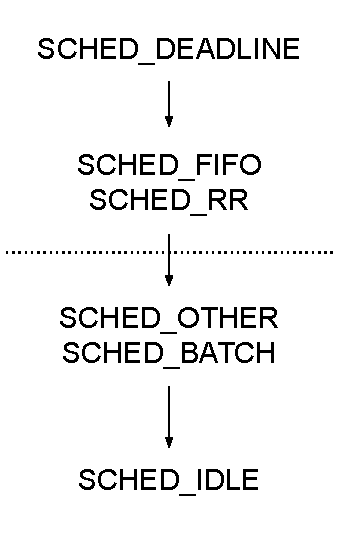
\includegraphics[width=\textwidth]{slides/realtime-linux-configuration/sched_precedence.pdf}
		\column{0.7\textwidth}
		\begin{itemize}
			\item When invoked, the scheduler looks for runnable tasks in a specific order
			\item \code{SCHED_FIFO} and \code{SCHED_RR} share the same \textbf{runqueue}
			\item However when a \code{SCHED_RR} task yields, any same prio \code{SCHED_FIFO} will run until done
			\item until \textbf{v6.6}, \code{SCHED_OTHER} and \code{SCHED_BATCH} uses the \textbf{C}ompletely \textbf{F}air \textbf{S}cheduler
			\item It was then replaced by \textbf{EEVDF} (Earliest Eligible Virtual Deadline First) Scheduler, improved in \textbf{v6.12}.
		\end{itemize}
	\end{columns}
\end{frame}

\begin{frame}
	\frametitle{Realtime Throttling}
	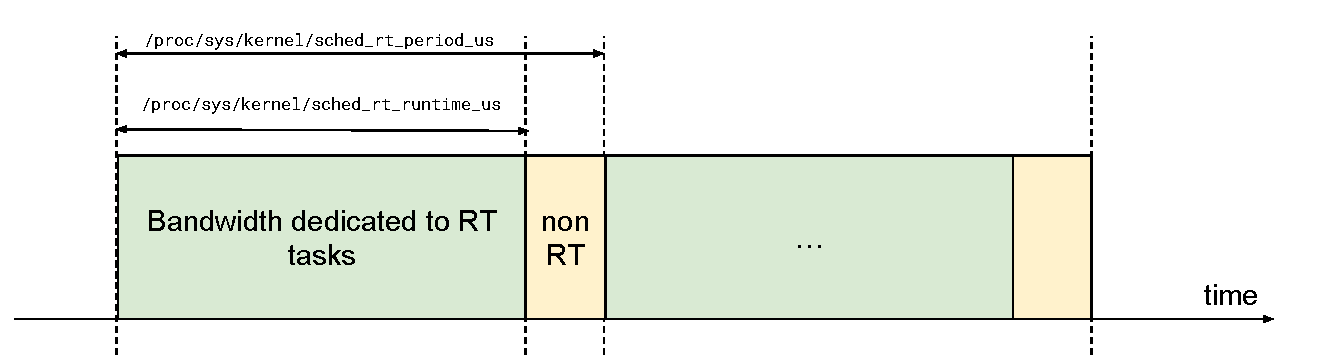
\includegraphics[width=0.9\textwidth]{slides/realtime-linux-configuration/rt_throttling.pdf}
	\begin{itemize}
		\item An infinite loop in a high-priority task will starve everything else
		\item \code{/proc/sys/kernel/sched_rt_period_us} : Time sharing period (\code{-1} to disable)
		\item \code{/proc/sys/kernel/sched_rt_runtime_us} : Amount of time in each period dedicated to RT tasks
		\item The default values allocates 95\% of the CPU time to RT tasks
		\item Can be used \textbf{per-cgroup}
	\end{itemize}
\end{frame}

\begin{frame}
	\frametitle{Deadline Server}
	\begin{itemize}
		\item RT Throttling can be overkill, as it fires even when no non-RT tasks needs to run
		\item The Deadline Server is a more precise replacement mechanism
		\item Uses a dedicated \code{SCHED_DEADLINE} task, the \textbf{deadline server}
		\item Available in \textbf{v6.12}, configurable in \textbf{debugfs}
		\item Won't trigger if there's no starving non-realtime task
		\item The starving task will only use the bandwidth it needs
		\item Replaces the old throttling mechanism, except for \textbf{grouping}
	\end{itemize}
\end{frame}

% System ticks and NOHZ
\begin{frame}
	\frametitle{System timer}
	\begin{itemize}
		\item The Scheduler is invoked on a regular basis to perform time-sharing activities
		\item This is sequenced through the \textbf{system ticks}, generated by a high resolution timer
		\item Several policies regarding system ticks are available:
		\item \kconfig{CONFIG_HZ_PERIODIC}: Always tick at a given rate. This introduces small interferences but is deterministic.
		\item \kconfig{CONFIG_NO_HZ_IDLE}: Disable the tick when idle, for powersasving
			\begin{itemize}
				\item Longer wakeup from Idle, replay the missed ticks (\textbf{jiffies} housekeeping)
			\end{itemize}
		\item \kconfig{CONFIG_NO_HZ_FULL}: Actively disables ticking even when not idle.
			\begin{itemize}
				\item Per-CPU setting, through the \code{nohz_full=<range>} boot parameter
				\item Only relevant on multi-core systems, one core must stay in nohz\_idle mode
				\item \code{nohz_full} cores will automatically offload their \textbf{RCU}
				\item Slightly more expensive Kernel to User transitions
			\end{itemize}
	\end{itemize}
\end{frame}

\begin{frame}
	\frametitle{System timer}
	\begin{columns}
		\column{0.7\textwidth}
	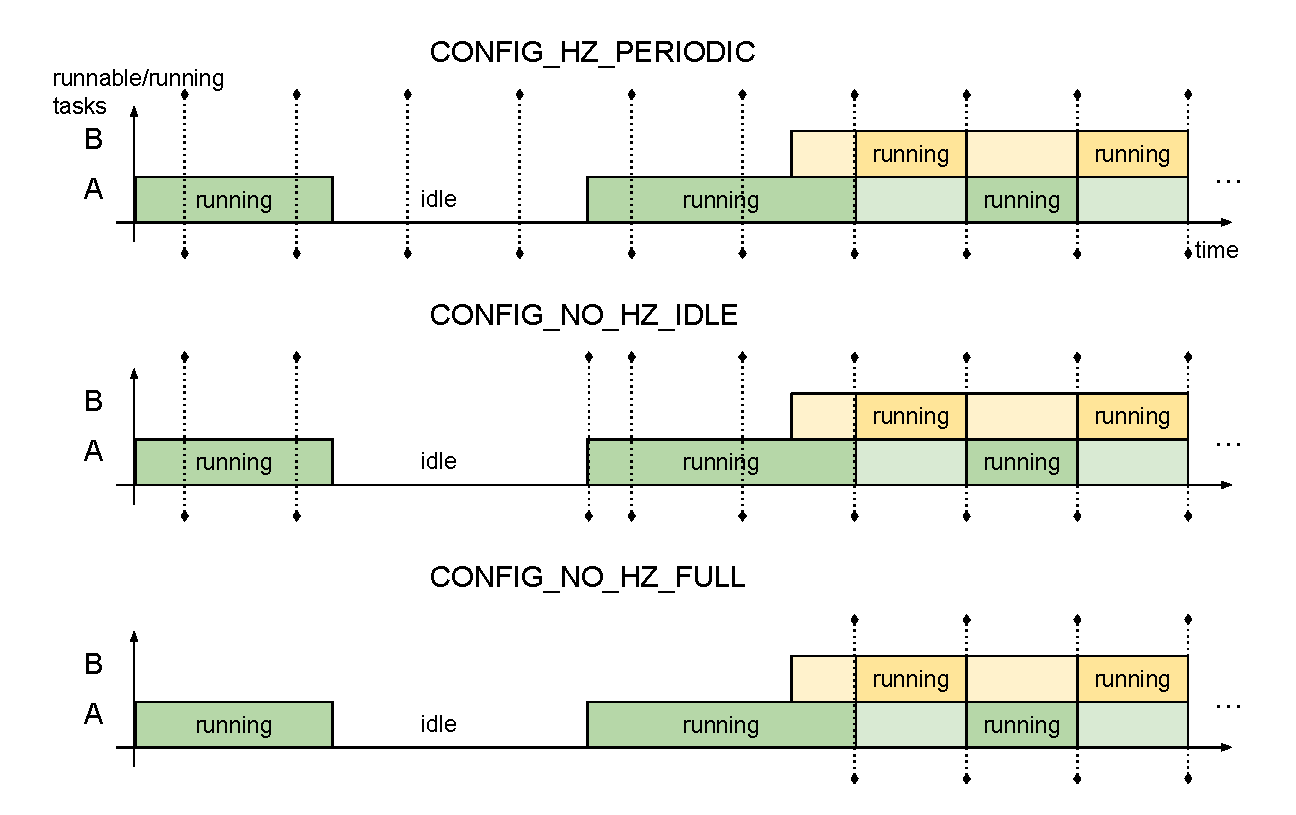
\includegraphics[width=\textwidth]{slides/realtime-linux-configuration/hz.pdf}
		\column{0.3\textwidth}
		\begin{itemize}
			\item Tick always enabled \\
				\vspace{1.3cm}
			\item Tick disabled in Idle \\
				\vspace{1.3cm}
			\item Tick disabled in Idle and when only one runnable task
		\end{itemize}
	\end{columns}
\end{frame}


% Memory management and allocators

% Writing a driver
\begin{frame}
		\frametitle{Writing a driver}
A few considerations can be taken when writing a driver
		\begin{itemize}
			\item Avoid using \ksym{raw_spinlock_t} unless really necessary
			\item Avoid forcing non-threaded interrupts, unless writing a driver involved in interrupt dispatch
				\begin{itemize}
					\item irqchip, gpio-irq drivers
					\item cpufreq and cpuidle drivers due to scheduler interaction
				\end{itemize}
			\item Beware of DMA bus mastering and other serialized IO buffering
				\begin{itemize}
					\item Certain register writes are buffered until the next register read
				\end{itemize}
		\end{itemize}
\end{frame}
